
\subsection{Ergebnisse}

Die Kopforientierung wird auf Basis verschiedener Sensordaten bestimmt.
Die aus unterschiedlichen Kombinationen der Sensoren berechneten Orientierungen stehen als Ausgabe zur Verfügung:
\begin{itemize}
  \item Marker-Tracking
  \item Gyroskop + Beschleunigungssensor
  \item Gyroskop + Beschleunigungssensor + Magnetometer
  \item Gyroskop + Beschleunigungssensor + Magnetometer + Marker-Tracking
\end{itemize}

Durch Einsatz des \ac{ROS}-Frameworks und durchgängige Verwendung des Transformationsbaums (vgl. Abs. \ref{headtracking_markerfusion_subsubsec}) ist dabei das Referenz-Koordinatensystem frei wählbar.
In der Visualisierung (s. Abb. \ref{fig:kopf_orientierung_rviz}) können die gewünschten Berechnungsergebnisse vom Benutzer ausgewählt werden.


Die Applikation konnte erfolgreich im unbewegten \emph{CoCar} getestet werden.
Tests im bewegten Fahrzeug sind noch durchzuführen.


\begin{figure}
  \centering
  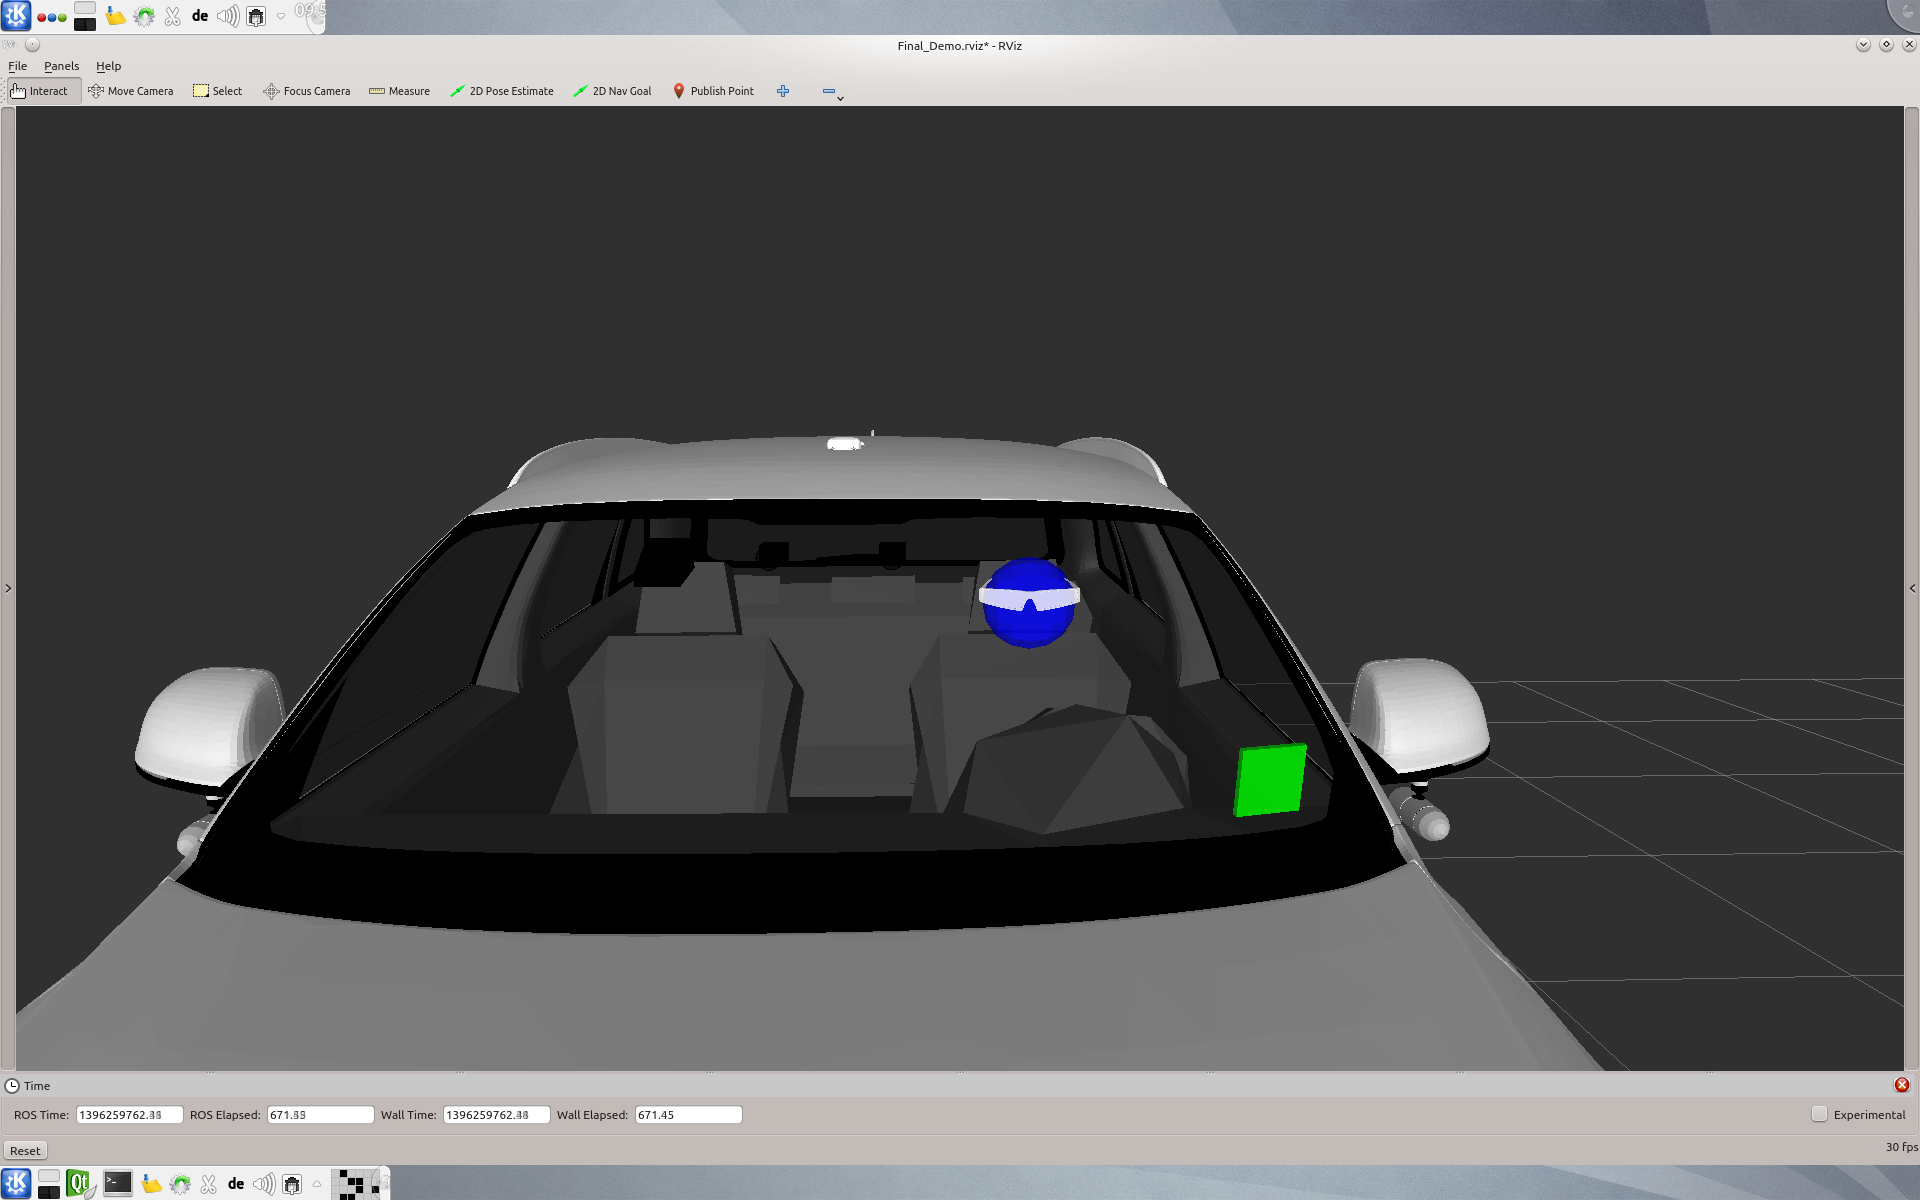
\includegraphics[width=0.4\textwidth]{Frontsicht_Kopf_Brille_RVIZ}
  \caption{Visualisierung der Kopforientierung}
  \label{fig:kopf_orientierung_rviz}
\end{figure}


\subsection{Ausblick}

%\todo[inline]{Irgendwie stimmen ab hier die Absatz-Abstände nicht mehr. Liegt das an der transformations-figure*?} % Ok, stimmen irgendwie doch wieder^^

Für Weiterentwicklungen des Systems bieten sich interessante Bereiche an:

Das System ist derzeit beschränkt auf die Bestimmung der Kopforientierung.
Eine Erweiterung, sodass zusätzlich auch die Position des Kopfes geschätzt wird, ist sicherlich der interessanteste Ansatzpunkt.
Dazu ist eine Integration der Orientierungsdaten über die Zeit nötig.
Da von der in Abs. \ref{headtracking_markertracking_subsubsec} beschriebenen \alvar-Bibliothek auch --bisher nicht verwendete-- Positionsinformationen geliefert werden, kann voraussichtlich die Stützung durch Kameradaten zu großen Teilen unverändert übernommen werden.

Außerdem bietet \alvar \ eine Bundle-Funktionalität, die bisher noch nicht eingesetzt wird.
Damit können im Innenraum des Autos weitere Marker angebracht werden, sodass bei nahezu beliebiger Blickrichtung des Fahrers immer ein Marker im Kamerabild zu erkennen ist.
Die Korrektur der \ac{IMU}-Daten durch Kameradaten wäre damit nicht mehr auf eine Blickrichtung in Fahrtrichtung beschränkt.

Möglich ist auch eine weitere Untersuchung des in Abs. \ref{headtracking_facetracking_subsubsec} beschriebenen Face-Trackings.
Hier ist die Erstellung einer neuen Gesichtsmaske --mit \ac{AR}-Brille-- ein vielversprechender Ansatz.
%\todo[inline]{Ist das so? Es gibt doch einige Argumente dagegen. -> siehe Antwort im sourcecode}
% TR: Ich glaube schon, dass es ein Ansatz ist, den man nochmal tiefer angehen könnte. Angeblich funktioniert der bisherige Face-Tracker auch mit normalen Brillen; sprich mit Spiegelung kann er umgehen. Von daher ist der Hauptgrund, dass es bei uns nicht auf Anhieb geklappt hat, wahrscheinlich die falsche Maske. Oder würdest du/ihr das hier raus nehmen?

Ein Ausbau der Hardware-Kompatibilität auf weitere Brillenmodelle wie beispielsweise \emph{Google Glass, Oculus Rift} \oae erscheint ebenfalls interessant.


